\documentclass{article}
\usepackage{amsmath, amsthm, amssymb, amsfonts}
\usepackage{thmtools}
\usepackage{graphicx}
\usepackage{setspace}
\usepackage{geometry}
\usepackage{float}
\usepackage{hyperref}
\usepackage[utf8]{inputenc}
\usepackage[english]{babel}
\usepackage{framed}
\usepackage[dvipsnames]{xcolor}
\usepackage{tcolorbox}
\usepackage{ dsfont }

\colorlet{LightGray}{White!90!Periwinkle}
\colorlet{LightOrange}{Orange!15}
\colorlet{LightGreen}{Green!15}

\graphicspath{ {./pictures/} }

\newcommand{\HRule}[1]{\rule{\linewidth}{#1}}

% ------------------------------------------------------------------------------

\begin{document}

% ------------------------------------------------------------------------------
% Cover Page and ToC
% ------------------------------------------------------------------------------

\title{ \normalsize \textsc{}
		\\ [2.0cm]
		\HRule{1.5pt} \\
		\LARGE \textbf{\uppercase{ Title }
        \HRule{2.0pt} \\ [0.6cm] \LARGE{ Subtitle } \vspace*{10\baselineskip}}
		}
\date{date}
\author{\textbf{} \\
		Gruppe:  \\
		Tutor:  }

\maketitle
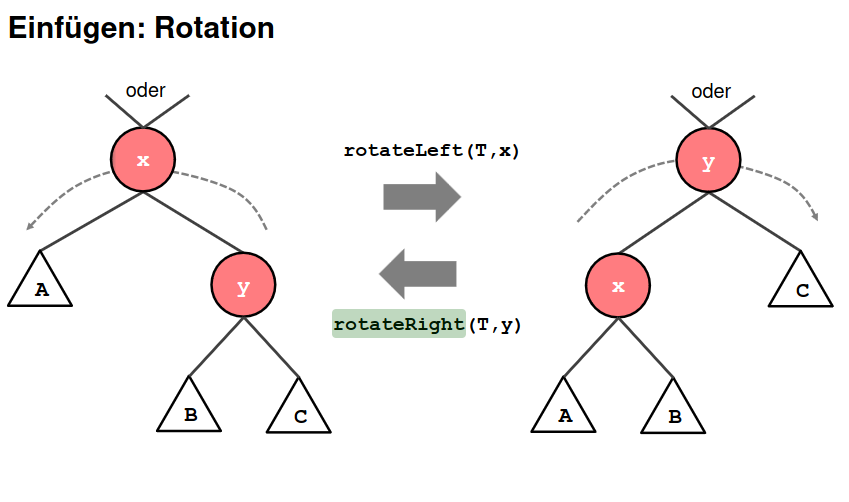
\includegraphics[scale=0.5]{ r } \\ 
\bigskip
rotateRight(T, y) 

\noindent x=y.left \\
y.left = x.right;
if x.right != nil THEN \\ 
    \indent x.right.parent = y; \\ 
x.parent = y.parent; \\ 
if y.parent==T.sent THEN \\ 
    \indent T.root = x; \\ 
ELSE \\ 
\indent IF y==y.parent.right THEN \\
\indent \indent y.parent.right = x; \\ 
\indent ELSE \\ 
\indent \indent y.parent.left = x; \\ 
x.right=y; \\ 
y.parent = x;  
\end{document}

